\section{Semiconductor Physics}

\qcontributor{Regina Eckert}

Generally, semiconductors are crystalline solids bonded into a lattice. In the Bohr model of the atom, the highest energy level (called the "valence" band) of an atom is considered filled when it contains 8 electrons (except the first energy level, which requires only 2 electrons). In semiconductors, atomic bonds completely "fill" the outer valence band of each atom, creating the semiconductor lattice.

	\begin{figure}[H]{
		\centering
		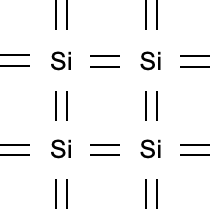
\includegraphics[width=0.2\textwidth]{n_led/si_lattice.png}
		\caption{Silicon Lattice}
		\vspace{-5mm}}
	\label{fig:SiLattice}
\end{figure}

Silicon has 4 electrons in its valence band. An electrons shared between two atoms creates a bond between those atoms. In the diagram above, a line between two silicon nuclei (designated by "Si", the symbol for silicon) represents an electron that is shared by those two silicon atoms. This electron is said to be in a "bond" between the atoms.

Sometimes, extra energy is added to the lattice. This extra energy can come from light hitting the semiconductor, like in solar cells or in digital cameras. The extra energy can also be from a voltage applied to the semiconductor, like in light-emitting diodes (LEDs). A bonded valence electron can absorb this energy. However, atomic bonds can only have a certain energy. This "excited" electron is now too energetic for the atomic bond. The excited electron can break free of the bond and move freely in the lattice. The process when light hits a semiconductor and excites an electron, breaking it free of its bond, is called the \textit{photovoltaic effect}.

When the electron breaks free of the atomic bond, it leaves a "hole" in the bond between two adjacent atoms. This hole has a positive charge because the negatively charged electron has left the bond. We can think of holes as "moving" in the semiconductor lattice, just as the electrons move. 

	\begin{figure}[H]{
		\centering
		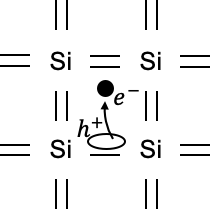
\includegraphics[width=0.2\textwidth]{n_led/si_lattice_wHole.png}
		\caption{Silicon lattice with electron $e^-$ in conduction band and hole $h^+$ where the bond is broken.}
		\vspace{-5mm}}
	\label{fig:SiLatticeWHole}
\end{figure}


Semiconductors can be visualized in terms of energy band diagrams that describe the bound ("valence band") and free ("conduction band") electrons in the semiconductor lattice. Valence band electrons have the particular energy allowed by the atomic bond, $E_V$. Conduction band electrons have minimum energy $E_C$. The energy difference between the valence and conduction bands is called the "band-gap energy", $E_G$, which is dependent on properties of the semiconductor.

	\begin{figure}[H]{
		\centering
		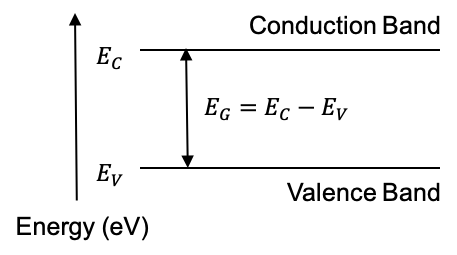
\includegraphics[width=0.4\textwidth]{n_led/band_diagram.png}
		\caption{Semiconductor energy band diagram}
		\vspace{-5mm}}
	\label{fig:BandDiagram}
\end{figure}

A conduction band electron with energy $E_C$ can recombine with a hole in the semiconductor lattice - that is, it can become a part of an atomic bond again. When this recombination happens, all of the energy that the electron has above the energy state of the valence band energy, $E_V$, gets emitted as a packet of energy. This energy can take the form of heat (a \textit{phonon}) or light (a \textit{photon}).

\subsection{Photons}
A photon is a discrete packet (or "quantum") of energy in the form of electromagnetic radiation. A photon has a particular frequency, $\nu$, of oscillation of the electromagnetic radiation. The frequency is inversely proportional to the photon's wavelength, $\lambda$. In vacuum, $\nu = \frac{c}{\lambda}$, where $c = 2.99\times10^8 m/s$ is the speed of light in a vacuum. The energy of a photon is given by $E = h\nu = \frac{hc}{\lambda}$, where $h = 4.136\times10^{-15} eV/Hz$ is Planck's constant.

Electromagnetic radiation with wavelengths between $380 ~\si{\nano\meter}$ and $700 ~\si{\nano\meter}$ (or $430-790 ~\si{\tera\hertz}$) is visible light, which can be perceived by human eyes. ($10^{12}~\si{\hertz} = 1~\si{\tera\hertz}$)

\subsection{Doping Semiconductors}

To control how current flows in a semiconductor, we have to manipulate the material's structure. We do this by "doping", or adding to, the material with other elements that have excess electrons or holes in comparison with the semiconductor.

For example, phosphorus (P) has 5 valence electrons compared to silicon's 4 valence electrons. It is added to silicon to add free electrons to the lattice, creating an "n-type" material. Similarly, we can dope semiconductors with elements that have less valence electrons than the semiconductor to make a lattice that has many holes (that is, empty electron bonds). This is called a "p-type" material. Boron (B), with 3 valence electrons, is a common p-type dopant for silicon.

It's important to note that because the elements we dope with are electrically neutral, n-type and p-type materials are also electrically neutral. That is, the material itself is not charged. This might be confusing, because we visualize n-type materials as having extra electrons and p-type materials as having extra holes, so we might think that they are negatively or positively charged. But because the number of protons and electrons is equal in a neutral element, the net charge of a doped material is still neutral. 

	\begin{figure}[H]{
		\centering
		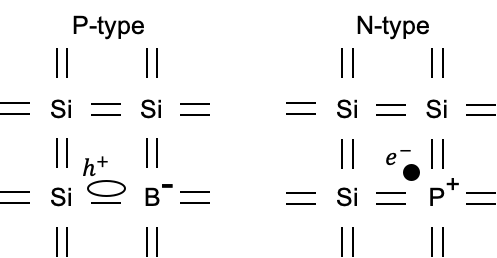
\includegraphics[width=0.4\textwidth]{n_led/doped_lattice.png}
		\caption{P-type and N-type doped lattices}
		\vspace{-5mm}}
	\label{fig:DopedSi}
\end{figure}
\iffalse
We can visualize how both holes and electrons move in the lattice in the figure below.
	\begin{figure}[H]{
		\centering
		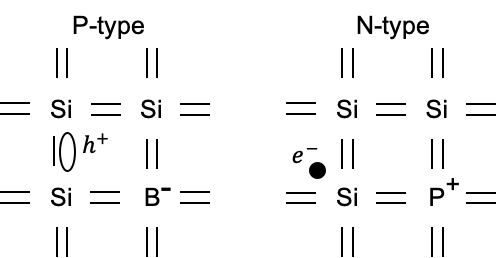
\includegraphics[width=0.4\textwidth]{n_led/doped_lattice_diffused.png}
		\caption{Movement of holes and electrons in P-type and N-type doped lattices}
		\vspace{-5mm}}
	\label{fig:DopedSi}
\end{figure}
\fi
\subsection{P-N Junction Diodes}

To create light-emitting diodes (LEDs), solar cells, and digital camera sensors, we fuse a p-type material that has a lot of extra holes in its lattice with an n-type material that has a lot of extra electrons. This is called a p-n junction diode. 

	\begin{figure}[H]{
		\centering
		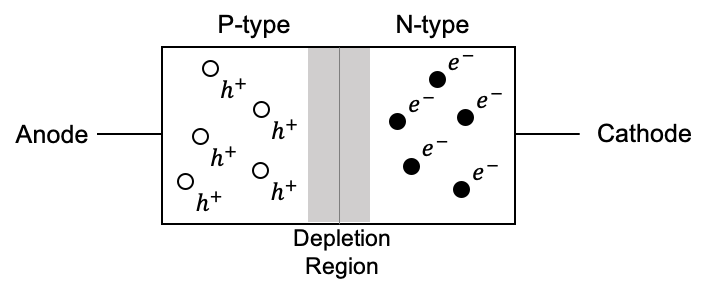
\includegraphics[width=0.5\textwidth]{n_led/pn_junction.png}
		\caption{P-N junction diode}
		\vspace{-5mm}}
	\label{fig:BandDiagramPhoton}
\end{figure}

When we first fuse the n- and p-type materials, the electrons and holes that are close to each other recombine and create a region called the "depletion region". In this region, there are no extra electrons or holes available and therefore current cannot flow across it without some help. 

When we apply a positive voltage to the p-type material (the "anode") relative to the n-type material (the "cathode"), electrons flow from the n-type to p-type material and the depletion region is decreased. This is because the electrons are attracted to the positive voltage applied at the anode and repelled by the negative voltage at the cathode. (And vice versa for the positive holes.) Current can flow across the device when this voltage is large enough that the insulating depletion region is gone. This is called a forward-bias and the diode is "on" in this case. 

However, if we apply a positive voltage to the n-type material, current does not flow. This is because the electrons are attracted to the positive voltage at the cathode, which pulls electrons out of the center of the p-n junction and increases the size of the depletion region. This means that current cannot flow across the device. In this case, the diode is "off" and no current flows from the anode to cathode.

\begin{figure}[H]{
	\centering
\begin{circuitikz} [american voltages]
	\draw
	(4,0) to[V,invert] (0,0) -- (0,2) 
	node[label={left:Anode}] {}
	to[D*,i=${I=I_d}$] (4,2)
	node[label={right:Cathode}] {}
	-- (4,0)
	;
\end{circuitikz}
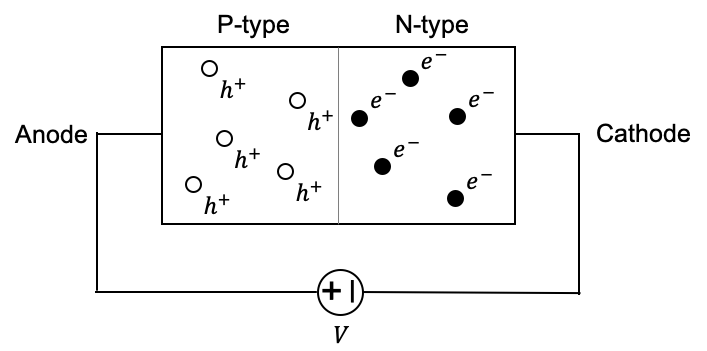
\includegraphics[width=0.4\textwidth]{n_led/pn_forward.png}
		\caption{P-N junction diode in ON state (forward-biased)}
\vspace{-5mm}}
\label{fig:pnJunctionOn}
\end{figure}

\begin{figure}[H]{
		\centering
		\begin{circuitikz} [american voltages]
			\draw
			
			(4,0) to[V] (0,0) -- (0,2) 
			node[label={left:Anode}] {}
			to[D*,i=${I=0A}$] (4,2)
			node[label={right:Cathode}] {}
			-- (4,0)
			;
		\end{circuitikz}
	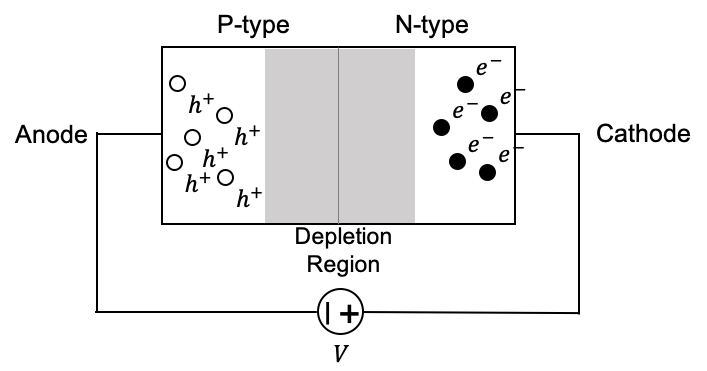
\includegraphics[width=0.4\textwidth]{n_led/pn_reverse.png}
		\caption{P-N junction diode in OFF state (reverse-biased)}
		\vspace{-5mm}}
	\label{fig:pnJunctionOff}
\end{figure}

\subsection{Light-Emitting Diodes}
LEDs are made of forward-biased p-n junction diodes. When the diode is on and current is flowing, electrons are moving across the p-n junction from the n-type through the p-type material to the anode. As they move, many electrons recombine with holes in the lattice. When this recombination happens, the electrons must emit their extra energy $E_G$ either as heat or light. LEDs are made of semiconductors that have properties such that this extra energy is more often released as light (\textit{photons}) than as heat. The photons emitted from an LED will have an energy that is equal to the band-gap energy of the semiconductor. Since a photon's energy is related to its frequency ($E=h\nu$), LED's are of specific, distinct colors determined by the semiconductor's band-gap.

Let's take a look at the energy band diagram for a recombination event. We can see that as an electron drops from the conduction band at energy $E_C$ to the valence band at energy $E_V$, it must emit energy equal to the band-gap, $E_G = E_C - E_V$. When light is emitted, $E_G$ is therefore the energy of the photon that is emitted.

	\begin{figure}[H]{
		\centering
		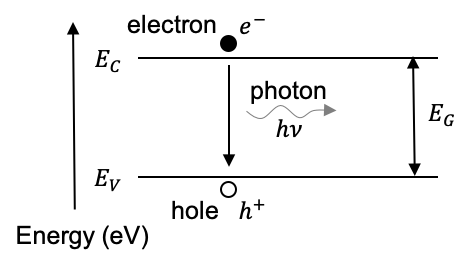
\includegraphics[width=0.4\textwidth]{n_led/band_diagram_photon.png}
		\caption{Semiconductor energy band diagram when recombination occurs and a photon is emitted}
		\vspace{-5mm}}
	\label{fig:BandDiagramPhoton}
\end{figure}
